% !TEX program = pdflatex
% ============================================================================
%   A Beginner-Friendly Walkthrough of the JPS4 Snake-Game Project
%   Companion document to the code under /src/Snake Game Code
%   Build: pdflatex project_guide.tex  (run twice for TOC)
% ============================================================================
\documentclass[11pt,a4paper]{article}

\usepackage[utf8]{inputenc}
\usepackage[T1]{fontenc}
\usepackage{lmodern}
\usepackage[margin=1in]{geometry}
\usepackage{microtype}
\usepackage{xcolor}
\usepackage{graphicx}
\usepackage{booktabs}
\usepackage{enumitem}
\usepackage{amsmath,amssymb}
\usepackage{tikz}
\usetikzlibrary{positioning,arrows.meta,calc,shapes.geometric,fit,backgrounds,decorations.pathreplacing,trees}
\usepackage{listings}
\usepackage{caption}
\usepackage{tcolorbox}
\tcbuselibrary{skins,breakable}
\usepackage[colorlinks=true,linkcolor=blue!55!black,urlcolor=blue!55!black,citecolor=blue!55!black]{hyperref}
\usepackage{titlesec}

% ---------------------- styling ---------------------------------------------
\definecolor{accent}{HTML}{1F4E79}
\definecolor{accent2}{HTML}{C0504D}
\definecolor{soft}{HTML}{F2F2F2}
\definecolor{soft2}{HTML}{EAF1F8}
\definecolor{wall}{HTML}{3B3B3B}
\definecolor{freecell}{HTML}{FFFFFF}
\definecolor{startc}{HTML}{2E7D32}
\definecolor{goalc}{HTML}{C62828}
\definecolor{visitedc}{HTML}{BBDEFB}
\definecolor{pathc}{HTML}{FFD54F}
\definecolor{jumpc}{HTML}{9C27B0}

\titleformat{\section}{\color{accent}\Large\bfseries}{\thesection.}{0.6em}{}
\titleformat{\subsection}{\color{accent}\large\bfseries}{\thesubsection}{0.5em}{}
\titleformat{\subsubsection}{\color{accent2}\normalsize\bfseries}{}{0pt}{}

\newtcolorbox{keybox}[1][]{enhanced,
  colback=soft2,colframe=accent,boxrule=0.4pt,
  arc=2pt,left=8pt,right=8pt,top=6pt,bottom=6pt,
  title={#1},coltitle=white,fonttitle=\bfseries,
  attach boxed title to top left={xshift=8pt,yshift=-6pt},
  boxed title style={colback=accent,boxrule=0pt,arc=1pt}}

\newtcolorbox{warnbox}[1][]{enhanced,
  colback=red!5,colframe=accent2,boxrule=0.4pt,
  arc=2pt,left=8pt,right=8pt,top=6pt,bottom=6pt,
  title={#1},coltitle=white,fonttitle=\bfseries,
  attach boxed title to top left={xshift=8pt,yshift=-6pt},
  boxed title style={colback=accent2,boxrule=0pt,arc=1pt}}

\lstset{
  basicstyle=\ttfamily\footnotesize,
  keywordstyle=\color{accent}\bfseries,
  commentstyle=\color{gray}\itshape,
  stringstyle=\color{accent2},
  showstringspaces=false,
  breaklines=true,
  frame=single,
  framerule=0.3pt,
  rulecolor=\color{gray!40},
  backgroundcolor=\color{soft},
  language=Python,
  xleftmargin=8pt,
  framexleftmargin=4pt
}

% --------------------- grid-drawing macros ----------------------------------
% \gridbase{n}{m}  draws an n-wide, m-tall grid outline
\newcommand{\gridbase}[2]{%
  \draw[step=0.6,gray!50,very thin] (0,0) grid (#1*0.6,#2*0.6);
  \draw[black,thick] (0,0) rectangle (#1*0.6,#2*0.6);
}
% \cellfill{col}{row}{color}   (row counted from TOP = 0)
% We'll pass maxrows so row is translated; simpler: use y-coord directly in caller.
\newcommand{\fillcell}[3]{%
  \fill[#3] (#1*0.6,#2*0.6) rectangle ({(#1+1)*0.6},{(#2+1)*0.6});
  \draw[gray!50,very thin] (#1*0.6,#2*0.6) rectangle ({(#1+1)*0.6},{(#2+1)*0.6});
}
\newcommand{\celltext}[3]{%
  \node at ({(#1+0.5)*0.6},{(#2+0.5)*0.6}) {\footnotesize #3};
}

% ============================================================================
\title{\vspace{-1.2cm}\color{accent}\textbf{A Beginner's Walkthrough}\\[2pt]
\large of the \emph{JPS4 Snake-Game Benchmark} Project\\[6pt]
{\normalsize Dijkstra, A*, and Jump Point Search for 4-Connected Grids}}
\author{Companion guide for the ADA course project\\
\small Jazib Waqas \textperiodcentered\ Salman Adnan \textperiodcentered\ Hunain Abbas}
\date{\today}

% ============================================================================
\begin{document}
\maketitle
\thispagestyle{empty}

\begin{center}
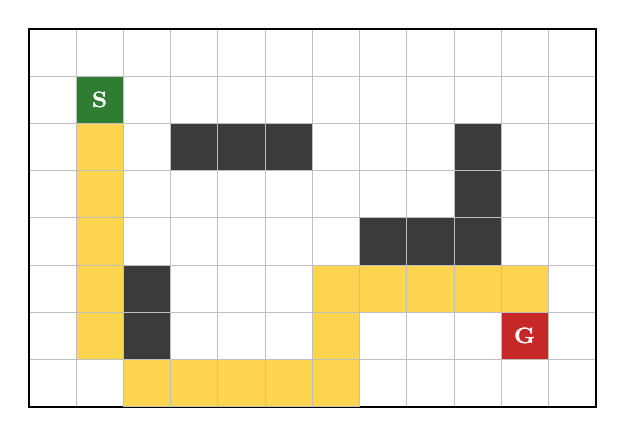
\begin{tikzpicture}[scale=1]
  \gridbase{12}{8}
  % walls
  \foreach \c in {3,4,5} { \fillcell{\c}{5}{wall} }
  \foreach \c in {7,8} { \fillcell{\c}{3}{wall} }
  \fillcell{9}{5}{wall}\fillcell{9}{4}{wall}\fillcell{9}{3}{wall}
  \fillcell{2}{2}{wall}\fillcell{2}{1}{wall}
  % start / goal
  \fillcell{1}{6}{startc}\celltext{1}{6}{\textcolor{white}{\textbf{S}}}
  \fillcell{10}{1}{goalc}\celltext{10}{1}{\textcolor{white}{\textbf{G}}}
  % path
  \foreach \c/\r in {1/5,1/4,1/3,1/2,1/1,2/0,3/0,4/0,5/0,6/0,6/1,6/2,7/2,8/2,9/2,10/2} {\fillcell{\c}{\r}{pathc}}
  \celltext{1}{6}{\textcolor{white}{\textbf{S}}}
  \celltext{10}{1}{\textcolor{white}{\textbf{G}}}
\end{tikzpicture}

\vspace{4pt}\small
\textit{From start (S) to goal (G), avoiding walls. That's the whole problem --- and it's the core of three famous algorithms.}
\end{center}

\vspace{1em}
\tableofcontents
\clearpage

% ============================================================================
\section*{Preface: How to read this document}
\addcontentsline{toc}{section}{Preface}

This guide assumes \textbf{zero prior knowledge}. You do not need to know what a graph is, what an algorithm is, or what Python looks like. Every new term is introduced the first time it appears, with a small picture whenever possible.

The document is organised like a staircase. Each section builds on the one before:

\begin{enumerate}[leftmargin=20pt,itemsep=2pt]
  \item First, we define the problem in plain English (\S\ref{sec:problem}).
  \item Then, we introduce the ideas (graph, priority queue, heuristic) that all three algorithms share (\S\ref{sec:blocks}).
  \item Next, we walk through each algorithm in turn --- Dijkstra, A*, and JPS4 --- with pictures showing exactly which cells the algorithm touches and why (\S\ref{sec:dijk}--\S\ref{sec:jps}).
  \item Then, we summarise the research paper the project is based on (\S\ref{sec:paper}).
  \item Finally, we open the project itself: every file, every class, every function, and how they connect (\S\ref{sec:arch}--\S\ref{sec:bench}).
\end{enumerate}

\begin{keybox}[How to use this in one sentence]
If any page is confusing, go back one section --- this document is designed so that nothing is used before it has been explained.
\end{keybox}

\clearpage

% ============================================================================
\section{What problem are we solving?}\label{sec:problem}

\subsection{The plain-English version}

Imagine a chessboard with some squares blocked by walls. You are standing on one square (the \textbf{start}, marked \textbf{S}). You want to reach another square (the \textbf{goal}, marked \textbf{G}). You can only move one step at a time, and only in four directions: up, down, left, right. You cannot step diagonally and you cannot walk through walls.

\begin{center}
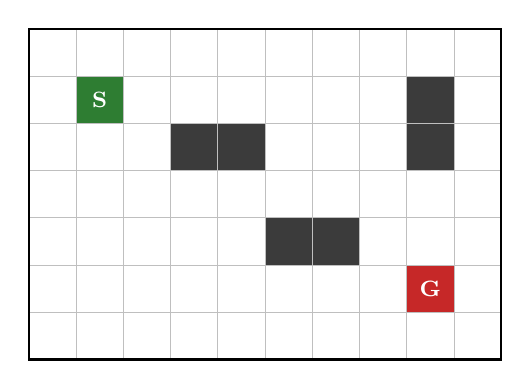
\begin{tikzpicture}[scale=1]
  \gridbase{10}{7}
  \foreach \c in {3,4} { \fillcell{\c}{4}{wall} }
  \foreach \c in {5,6} { \fillcell{\c}{2}{wall} }
  \fillcell{8}{5}{wall}\fillcell{8}{4}{wall}
  \fillcell{1}{5}{startc}\celltext{1}{5}{\textcolor{white}{\textbf{S}}}
  \fillcell{8}{1}{goalc}\celltext{8}{1}{\textcolor{white}{\textbf{G}}}
\end{tikzpicture}
\end{center}

\noindent The question is: \textbf{what is the shortest route from S to G?}

That's it. That is the entire problem. It sounds easy because a human can glance at a small grid and see a good route almost instantly. Computers cannot. A computer has to check squares one at a time, and on a big grid it has to check a \textit{lot} of them --- possibly tens of thousands. How it decides \textit{which squares to check first} is what makes an algorithm fast or slow.

\subsection{Why anyone cares}

This problem sounds like a puzzle, but it appears everywhere:

\begin{itemize}[leftmargin=20pt,itemsep=2pt]
  \item \textbf{Video games.} In almost every game with characters that walk around, there is a pathfinder running behind the scenes. When a monster chases you in a dungeon, something like this is deciding where it steps next.
  \item \textbf{Robotics.} A delivery robot inside a warehouse needs to get from shelf A to shelf B without bumping into shelves or other robots.
  \item \textbf{Navigation apps.} Google Maps is a fancier cousin of this problem, on a road network instead of a grid.
  \item \textbf{Logistics.} Routing trucks, planning forklift movements, scheduling crane moves in a shipping yard.
\end{itemize}

\subsection{What makes a grid a ``grid graph''}

When a computer scientist looks at our board, they don't see squares --- they see a \emph{graph}. A graph is just a collection of \textbf{nodes} (dots) connected by \textbf{edges} (lines). Each free square becomes one dot, and we draw a line between two dots whenever you can walk directly from one square to the other (so: adjacent, free, not separated by a wall).

\begin{center}
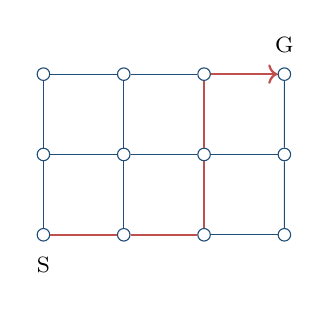
\begin{tikzpicture}[scale=0.85, every node/.style={font=\footnotesize}]
  \foreach \x in {0,1,2,3} \foreach \y in {0,1,2} {
    \node[circle,draw=accent,fill=white,inner sep=1.6pt] (n\x\y) at (\x*1.2,\y*1.2) {};
  }
  % edges (horizontal)
  \foreach \x/\xn in {0/1,1/2,2/3} \foreach \y in {0,1,2} {
    \draw[accent] (n\x\y) -- (n\xn\y);
  }
  \foreach \x in {0,1,2,3} \foreach \y/\yn in {0/1,1/2} {
    \draw[accent] (n\x\y) -- (n\x\yn);
  }
  \node[below=2pt of n00] {S};
  \node[above=2pt of n32] {G};
  \draw[->,thick,accent2] (n00) -- (n10) -- (n20) -- (n21) -- (n22) -- (n32);
\end{tikzpicture}
\end{center}

\noindent Every step is an edge. Every edge has the same \emph{cost}: 1. So the ``shortest path'' is the path with the fewest steps. Because every step costs the same, we call this a \textbf{uniform-cost 4-connected grid graph}. Memorise that phrase; it's the exact setting all three algorithms are built for.

\subsection{The two things we measure}

Whenever we compare algorithms in this project, we measure two numbers:

\begin{keybox}[The two metrics]
\textbf{(1) Node expansions} --- how many grid cells the algorithm ``looked at'' (pulled out of its to-do list to process). This is a pure count, independent of the machine.\\[2pt]
\textbf{(2) Search time} --- actual wall-clock time in milliseconds. This depends on the machine and the programming language.
\end{keybox}

\noindent Expansions are the cleaner number because they reflect the \textit{algorithm}, not the computer. Search time is what the user eventually experiences, but it's noisy.

\clearpage
% ============================================================================
\section{Building blocks shared by all three algorithms}\label{sec:blocks}

All three algorithms we study --- Dijkstra, A*, and JPS4 --- share the same skeleton. They differ only in three knobs, which we'll identify at the end of this section. First let's build the skeleton.

\subsection{The ``frontier'' idea}

Imagine standing at S and gradually exploring outward. At any moment, there are some squares you have already visited, and some squares that are on the \emph{border} between the explored region and the unknown. That border is called the \textbf{frontier} (or ``open list'').

At every step the algorithm does one thing: \textit{pick one square from the frontier, mark it visited, and add its free neighbours to the frontier}. Repeat until the goal pops out.

\begin{center}
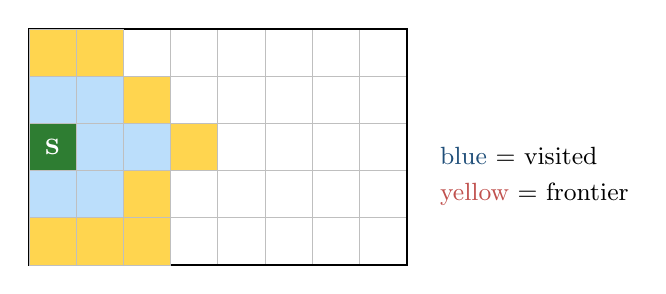
\begin{tikzpicture}[scale=1]
  \gridbase{8}{5}
  \foreach \c/\r in {0/2,1/2,2/2,0/3,1/3,0/1,1/1} {\fillcell{\c}{\r}{visitedc}}
  \foreach \c/\r in {2/3,2/1,0/0,1/0,2/0,0/4,1/4,3/2} {\fillcell{\c}{\r}{pathc}}
  \fillcell{0}{2}{startc}\celltext{0}{2}{\textcolor{white}{\textbf{S}}}
  \node[right=0.3cm] at (8*0.6,2.3*0.6) {\small \textcolor{accent}{blue} = visited};
  \node[right=0.3cm] at (8*0.6,1.5*0.6) {\small \textcolor{accent2}{yellow} = frontier};
\end{tikzpicture}
\end{center}

\noindent The cleverness is in \emph{which} frontier cell you pick next. That one decision is the whole story.

\subsection{The priority queue}

The frontier is not a plain list. It is a \textbf{priority queue}: a container where every item has a number attached (a ``priority''), and whenever you ask for an item you always get the one with the smallest number.

A good mental picture: a pile of sticky notes, each with a number. You always pick the one with the smallest number off the top of the pile. Inserting a new note is cheap, and so is removing the smallest.

\begin{keybox}[Why a priority queue?]
Different algorithms will attach different priority numbers to each frontier cell. The priority queue doesn't care what the number \emph{means} --- it just gives you the smallest one. That is how the \emph{same skeleton} can behave like three different algorithms, simply by choosing a different priority formula.
\end{keybox}

In the project's code (\texttt{helper.py}), the priority queue is Python's built-in \texttt{heapq}, and each frontier entry is a \texttt{SearchNode} object holding the priority, the running cost, the cell, and a back-pointer to the parent cell.

\subsection{Cost so far: \texorpdfstring{$g$}{g}}

For every cell we visit, we record \textbf{how many steps it took to get there from S}. That number is called $g$ (for ``cost so far''). The start has $g=0$; its neighbours have $g=1$; their neighbours have $g=2$; and so on.

\subsection{Estimated cost to go: \texorpdfstring{$h$}{h}}

Some algorithms also want to \emph{guess} how far the goal still is from a given cell. That guess is called $h$ (for ``heuristic''). In a 4-connected grid, a very good guess is the \textbf{Manhattan distance}:

\begin{center}
$h(\text{cell}) = |{\text{cell}.x - \text{goal}.x}| + |{\text{cell}.y - \text{goal}.y}|$
\end{center}

That is: pretend there are no walls and count the minimum number of cardinal steps you would need. Because you can't do better than that (walls only make things harder), Manhattan distance is \emph{never an overestimate} --- a property called \textbf{admissibility}. Admissibility is the magic ingredient that lets A* still guarantee the shortest path even though it is guessing.

\begin{center}
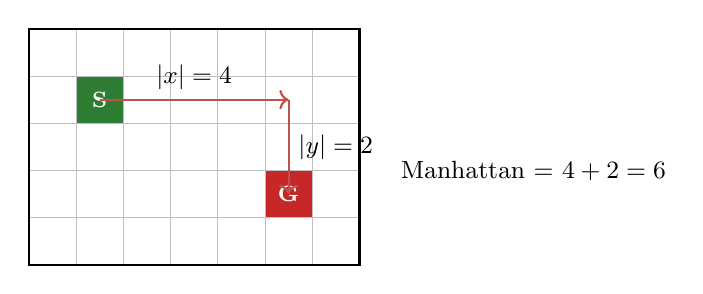
\begin{tikzpicture}[scale=1]
  \gridbase{7}{5}
  \fillcell{1}{3}{startc}\celltext{1}{3}{\textcolor{white}{\textbf{S}}}
  \fillcell{5}{1}{goalc}\celltext{5}{1}{\textcolor{white}{\textbf{G}}}
  \draw[->,thick,accent2] (1.5*0.6,3.5*0.6) -- (5.5*0.6,3.5*0.6);
  \draw[->,thick,accent2] (5.5*0.6,3.5*0.6) -- (5.5*0.6,1.5*0.6);
  \node[above] at (3.5*0.6,3.5*0.6) {\small $|x|=4$};
  \node[right] at (5.5*0.6,2.5*0.6) {\small $|y|=2$};
  \node[right=0.4cm] at (7*0.6,2*0.6) {\small Manhattan = $4+2 = 6$};
\end{tikzpicture}
\end{center}

\subsection{Total priority: \texorpdfstring{$f = g + h$}{f = g + h}}

The priority the algorithms use is a number called $f$, which is just $g + h$:

\begin{center}
$f(\text{cell}) = g(\text{cell}) + h(\text{cell})$
\end{center}

\noindent That is: ``how many steps we already spent to reach this cell, plus our best guess of how many more we'll need''. When the priority queue gives us the cell with the smallest $f$, it's giving us the cell that \emph{could} lie on the shortest path, because no other candidate currently looks cheaper.

\subsection{The three knobs}

Now we can describe the three algorithms in a single sentence each, by saying how they set those knobs:

\begin{center}
\renewcommand{\arraystretch}{1.25}
\begin{tabular}{@{}llll@{}}
\toprule
\textbf{Algorithm} & $h$ (heuristic) & \textbf{Successors (neighbours)} & \textbf{Priority} \\
\midrule
Dijkstra & always $0$ & all 4 cardinal neighbours & $f = g$ \\
A*       & Manhattan  & all 4 cardinal neighbours & $f = g + h$ \\
JPS4     & Manhattan  & only \emph{jump points} (see \S\ref{sec:jps}) & $f = g + h$ \\
\bottomrule
\end{tabular}
\end{center}

Three lines. That is literally the difference. In the code (\texttt{pathing\_grid.py}), the same function \texttt{astar\_jps} runs all three; it receives a \texttt{heuristic} function and a \texttt{successors} function as arguments, and the caller swaps them depending on which algorithm the user asked for.

\clearpage
% ============================================================================
\section{Dijkstra's algorithm}\label{sec:dijk}

\subsection{The idea in one sentence}

\emph{Spread out from the start in a perfectly circular ripple, one step at a time, until you hit the goal.}

Dijkstra does not use a heuristic. It has no idea where the goal is. It just processes cells in order of increasing distance from the start, like a water ripple. Because every cell at distance $d$ is processed before any cell at distance $d+1$, the very first time we pull the goal out of the priority queue, we know we've found the shortest path.

\subsection{A worked example}

Start at S. Its four neighbours all go into the frontier with $g=1$. We pick one (any one), process it, adding its unvisited neighbours with $g=2$. And so on.

\begin{center}
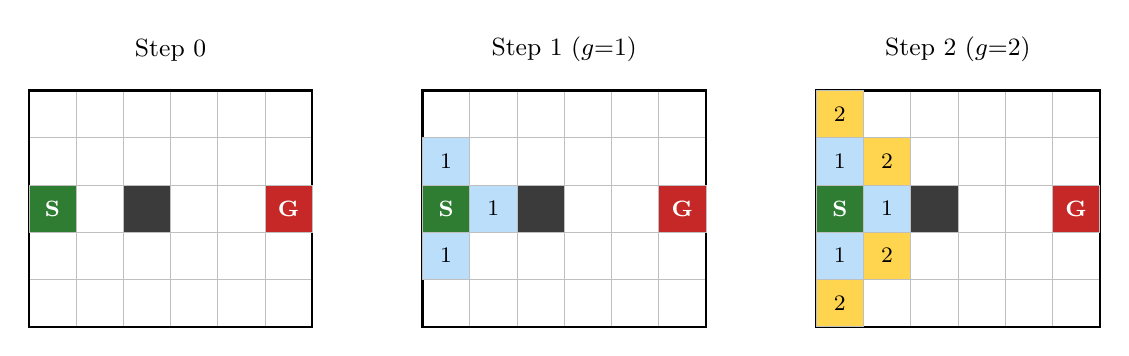
\begin{tikzpicture}[scale=1]
  \begin{scope}
    \node[above] at (3*0.6,5.4*0.6) {\small Step 0};
    \gridbase{6}{5}
    \foreach \c in {2} { \fillcell{\c}{2}{wall} }
    \fillcell{0}{2}{startc}\celltext{0}{2}{\textcolor{white}{\textbf{S}}}
    \fillcell{5}{2}{goalc}\celltext{5}{2}{\textcolor{white}{\textbf{G}}}
  \end{scope}

  \begin{scope}[xshift=5cm]
    \node[above] at (3*0.6,5.4*0.6) {\small Step 1 ($g{=}1$)};
    \gridbase{6}{5}
    \foreach \c in {2} { \fillcell{\c}{2}{wall} }
    \fillcell{0}{2}{startc}
    \fillcell{1}{2}{visitedc}\celltext{1}{2}{1}
    \fillcell{0}{1}{visitedc}\celltext{0}{1}{1}
    \fillcell{0}{3}{visitedc}\celltext{0}{3}{1}
    \celltext{0}{2}{\textcolor{white}{\textbf{S}}}
    \fillcell{5}{2}{goalc}\celltext{5}{2}{\textcolor{white}{\textbf{G}}}
  \end{scope}

  \begin{scope}[xshift=10cm]
    \node[above] at (3*0.6,5.4*0.6) {\small Step 2 ($g{=}2$)};
    \gridbase{6}{5}
    \foreach \c in {2} { \fillcell{\c}{2}{wall} }
    \foreach \c/\r in {0/1,0/3,1/2} {\fillcell{\c}{\r}{visitedc}}
    \foreach \c/\r in {1/1,1/3,0/0,0/4} {\fillcell{\c}{\r}{pathc}}
    \fillcell{0}{2}{startc}
    \celltext{0}{1}{1}\celltext{0}{3}{1}\celltext{1}{2}{1}
    \celltext{1}{1}{2}\celltext{1}{3}{2}\celltext{0}{0}{2}\celltext{0}{4}{2}
    \celltext{0}{2}{\textcolor{white}{\textbf{S}}}
    \fillcell{5}{2}{goalc}\celltext{5}{2}{\textcolor{white}{\textbf{G}}}
  \end{scope}
\end{tikzpicture}
\end{center}

\noindent After enough ripples, the goal is reached. Following the back-pointers from G back to S gives the shortest route.

\subsection{Pseudocode}
\begin{lstlisting}[language=Python]
def dijkstra(start, goal, grid):
    frontier = PriorityQueue()
    frontier.push((g=0, start))
    came_from = {start: None}
    best_g    = {start: 0}

    while not frontier.empty():
        g, cell = frontier.pop()     # smallest g first
        if cell == goal:
            return reconstruct(came_from, goal)
        for nb in cell.neighbours():        # four cardinal
            if nb is wall: continue
            new_g = g + 1
            if new_g < best_g.get(nb, inf):
                best_g[nb]   = new_g
                came_from[nb] = cell
                frontier.push((new_g, nb))
    return None   # unreachable
\end{lstlisting}

\subsection{What's good, what's not}

\begin{itemize}[leftmargin=20pt,itemsep=2pt]
  \item[\textcolor{accent}{\textbf{+}}] \textbf{Always correct.} It will find the shortest path every time, as long as one exists.
  \item[\textcolor{accent}{\textbf{+}}] \textbf{Conceptually simple.} Nothing fancy; no heuristic to tune.
  \item[\textcolor{accent2}{\textbf{--}}] \textbf{Wasteful.} It explores in \emph{every} direction, including directions pointing away from the goal. On a big map it may visit tens of thousands of cells before stumbling into G. This is the exact weakness A* was invented to fix.
\end{itemize}

\clearpage
% ============================================================================
\section{A* search}\label{sec:astar}

\subsection{The idea in one sentence}

\emph{Dijkstra, but bias the ripple so it grows faster in the direction of the goal.}

A* uses the Manhattan-distance heuristic $h$ to break ties. Instead of ordering the frontier by $g$ alone (``distance from start''), it orders by $f = g + h$ (``distance from start plus estimated distance to goal''). Cells that point toward G get a lower priority number and come out of the queue sooner. Cells that point away get pushed to the back.

The result: instead of a round ripple, A* expands in an elongated shape that stretches toward the goal.

\subsection{Dijkstra vs.\ A*, same grid, side by side}

Each coloured cell is one that the algorithm actually pulled out of the frontier (``expanded''). The darker the colour, the earlier it was expanded.

\begin{center}
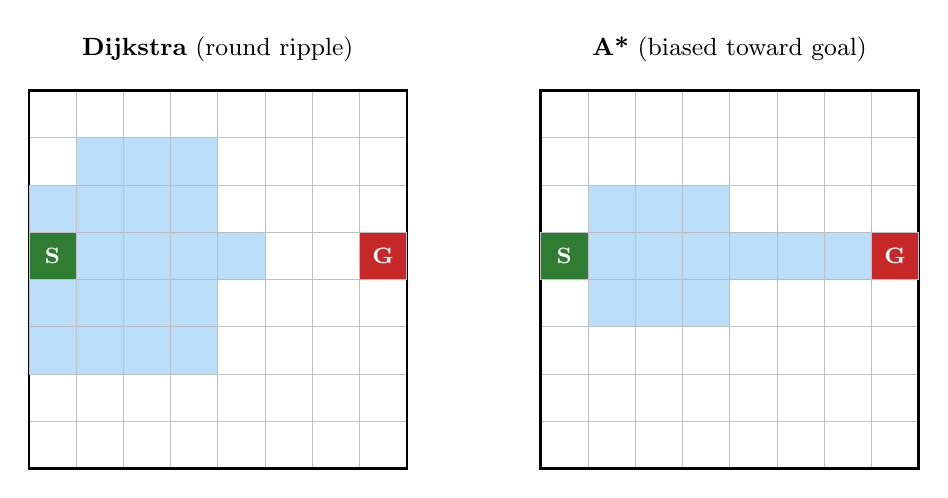
\begin{tikzpicture}[scale=1]
  \begin{scope}
    \node[above] at (4*0.6,8.4*0.6) {\small \textbf{Dijkstra} (round ripple)};
    \gridbase{8}{8}
    \foreach \c/\r in {0/3,0/4,1/3,1/4,1/5,2/3,2/4,2/5,0/2,2/2,3/4,3/5,1/6,1/2,0/5,3/6,2/6,3/3,3/2,4/4} {\fillcell{\c}{\r}{visitedc}}
    \fillcell{0}{4}{startc}\celltext{0}{4}{\textcolor{white}{\textbf{S}}}
    \fillcell{7}{4}{goalc}\celltext{7}{4}{\textcolor{white}{\textbf{G}}}
  \end{scope}
  \begin{scope}[xshift=6.5cm]
    \node[above] at (4*0.6,8.4*0.6) {\small \textbf{A*} (biased toward goal)};
    \gridbase{8}{8}
    \foreach \c/\r in {0/4,1/4,2/4,3/4,4/4,5/4,6/4,1/3,1/5,2/3,2/5,3/3,3/5} {\fillcell{\c}{\r}{visitedc}}
    \fillcell{0}{4}{startc}\celltext{0}{4}{\textcolor{white}{\textbf{S}}}
    \fillcell{7}{4}{goalc}\celltext{7}{4}{\textcolor{white}{\textbf{G}}}
  \end{scope}
\end{tikzpicture}
\end{center}

\noindent On an open map the difference is dramatic. Dijkstra expands dozens of cells it didn't need to; A* takes an almost-straight line.

\subsection{Why does adding $h$ still give the shortest path?}

This is the subtlety that made A* famous in 1968 (Hart, Nilsson, and Raphael). The argument is: as long as $h$ never \emph{over-estimates} the true remaining cost, the first time A* pops the goal out of the priority queue, the $g$ value attached to it is already optimal. Manhattan distance on a 4-connected grid is never an over-estimate (walls only make things harder), so we're safe.

\begin{keybox}[The rule for a safe heuristic]
$h(\text{cell}) \le$ actual shortest distance from cell to goal, \textit{for every cell}.\\
If that holds, A* is guaranteed to find the shortest path. This property is called \textbf{admissibility}.
\end{keybox}

\subsection{Pseudocode}
\begin{lstlisting}[language=Python]
def astar(start, goal, grid):
    frontier = PriorityQueue()
    frontier.push((f=h(start), g=0, start))
    came_from, best_g = {start: None}, {start: 0}

    while not frontier.empty():
        f, g, cell = frontier.pop()
        if cell == goal:
            return reconstruct(came_from, goal)
        for nb in cell.neighbours():
            if nb is wall: continue
            new_g = g + 1
            if new_g < best_g.get(nb, inf):
                best_g[nb]   = new_g
                came_from[nb] = cell
                frontier.push((new_g + h(nb), new_g, nb))
    return None
\end{lstlisting}

Notice that the only difference from Dijkstra is line by line identical \emph{except} the priority pushed into the queue: \texttt{new\_g + h(nb)} instead of just \texttt{new\_g}. That is the whole change.

\clearpage
% ============================================================================
\section{Jump Point Search for 4-connected grids (JPS4)}\label{sec:jps}

This is the most interesting algorithm in the project, and also the trickiest. Pay close attention to the setup --- the algorithm itself is short, but it only makes sense after you understand the \textbf{path-symmetry problem} it is designed to solve.

\subsection{The path-symmetry problem}

Look at a small open section of grid:

\begin{center}
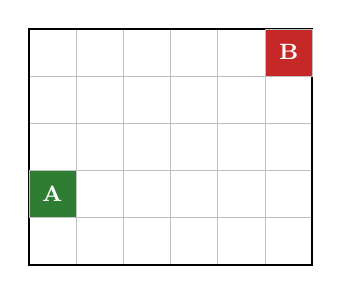
\begin{tikzpicture}[scale=1]
  \gridbase{6}{5}
  \fillcell{0}{1}{startc}\celltext{0}{1}{\textcolor{white}{\textbf{A}}}
  \fillcell{5}{4}{goalc}\celltext{5}{4}{\textcolor{white}{\textbf{B}}}
\end{tikzpicture}
\end{center}

\noindent How many shortest paths are there from A to B? The answer: \emph{very many}. Any sequence with 5 rights and 3 ups, in any order, is a valid shortest path. All of them have the same length (8). They are all \textit{equivalent} --- none is better than any other. A* will expand a lot of cells to compare these equivalent paths, even though it doesn't matter which one wins.

This duplication is called \textbf{path symmetry}. It is pure wasted work: if the grid is open, there is nothing to decide between the symmetric alternatives, so A* shouldn't even be looking at them.

\subsection{Canonical ordering: ``there is only one path''}

The fix is to pretend, artificially, that only one ordering is allowed. JPS4 picks a rule called \textbf{horizontal-first}: ``do all your horizontal steps before any vertical steps''. Under this rule, on an open map, there is exactly \emph{one} shortest path from A to B, not many:

\begin{center}
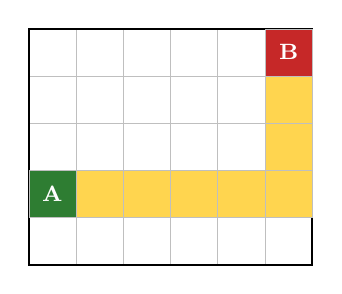
\begin{tikzpicture}[scale=1]
  \gridbase{6}{5}
  \foreach \c/\r in {1/1,2/1,3/1,4/1,5/1,5/2,5/3} {\fillcell{\c}{\r}{pathc}}
  \fillcell{0}{1}{startc}\celltext{0}{1}{\textcolor{white}{\textbf{A}}}
  \fillcell{5}{4}{goalc}\celltext{5}{4}{\textcolor{white}{\textbf{B}}}
\end{tikzpicture}
\end{center}

\noindent All the other shortest paths still exist in principle, but the algorithm refuses to consider them. This does not hurt optimality --- they all have the same length anyway.

\subsection{Natural neighbours and forced neighbours}

If every cell still produced four neighbours, the canonical ordering alone wouldn't help. JPS4 also \textbf{prunes} the neighbour list according to how you arrived at the current cell. The rules come straight from Baum (2025), Algorithm 2:

\begin{center}
\renewcommand{\arraystretch}{1.25}
\begin{tabular}{@{}ll@{}}
\toprule
\textbf{You arrived moving\ldots} & \textbf{Natural neighbours} \\
\midrule
Horizontally (left or right) & All three non-parent neighbours (forward, up, down) \\
Vertically (up or down)      & Only the one cell straight ahead in the same direction \\
\bottomrule
\end{tabular}
\end{center}

\begin{center}
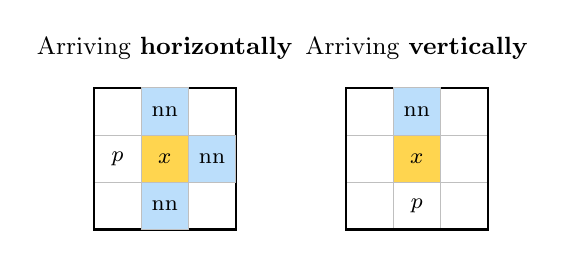
\begin{tikzpicture}[scale=1]
  % Horizontal movement, 3 naturals
  \begin{scope}
    \node[above] at (1.5*0.6,3.4*0.6) {\small Arriving \textbf{horizontally}};
    \gridbase{3}{3}
    \celltext{0}{1}{$p$}
    \fillcell{1}{1}{pathc}\celltext{1}{1}{$x$}
    \fillcell{2}{1}{visitedc}\celltext{2}{1}{nn}
    \fillcell{1}{2}{visitedc}\celltext{1}{2}{nn}
    \fillcell{1}{0}{visitedc}\celltext{1}{0}{nn}
  \end{scope}
  \begin{scope}[xshift=3.2cm]
    \node[above] at (1.5*0.6,3.4*0.6) {\small Arriving \textbf{vertically}};
    \gridbase{3}{3}
    \celltext{1}{0}{$p$}
    \fillcell{1}{1}{pathc}\celltext{1}{1}{$x$}
    \fillcell{1}{2}{visitedc}\celltext{1}{2}{nn}
  \end{scope}
\end{tikzpicture}
\end{center}

\noindent (Here $p$ is the parent cell we arrived from, $x$ is the current cell, and ``nn'' marks a natural neighbour.)

Now here's the catch: pruning so aggressively \emph{can} miss paths if there are obstacles. Look at this situation:

\begin{center}
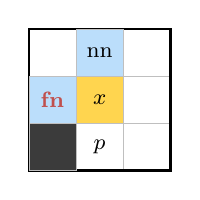
\begin{tikzpicture}[scale=1]
  \gridbase{3}{3}
  \celltext{1}{0}{$p$}
  \fillcell{1}{1}{pathc}\celltext{1}{1}{$x$}
  \fillcell{0}{0}{wall}
  \fillcell{0}{1}{visitedc}\celltext{0}{1}{\textcolor{accent2}{\textbf{fn}}}
  \fillcell{1}{2}{visitedc}\celltext{1}{2}{nn}
\end{tikzpicture}
\end{center}

\noindent We arrived at $x$ moving up. Normally we'd only keep the cell straight above $x$ (the ``nn''). But the cell to the left of $x$ (labelled \textbf{fn}, for \emph{forced neighbour}) has become interesting because the cell to the left of $p$ is a wall. If we don't expand left at $x$, there's no other way to get around that wall. So we add it back in as a \emph{forced} neighbour --- a neighbour that would normally be pruned but is needed because an obstacle broke the symmetry.

\begin{keybox}[The rule for forced neighbours (vertical movement)]
Moving vertically, check each of the two sideways neighbours of $x$ (left and right). If the corresponding sideways neighbour of $p$ is a \emph{wall}, then the one at $x$ becomes \textbf{forced}. (Horizontal movement never produces forced neighbours.)
\end{keybox}

\subsection{Jumping}

The final trick: instead of walking one step at a time, JPS4 \emph{skips ahead}. When moving vertically, it keeps stepping until one of three things happens:

\begin{enumerate}[leftmargin=20pt,itemsep=2pt]
  \item It hits a wall or the edge of the grid $\rightarrow$ dead end, stop.
  \item It reaches the goal $\rightarrow$ success, stop.
  \item It finds a cell that has a \emph{forced} neighbour $\rightarrow$ stop here; this cell is a \textbf{jump point} and must be added to the frontier.
\end{enumerate}

\noindent All the cells in between are silently skipped. They never enter the priority queue and never add to the expansion count. That is where the speed comes from.

Horizontal moves are handled slightly differently --- they advance just one step and always return the result. This asymmetry is the reason the algorithm is called \textbf{horizontal-first} JPS (HJPS) in Baum's paper.

\subsection{A visual intuition of jumping}

\begin{center}
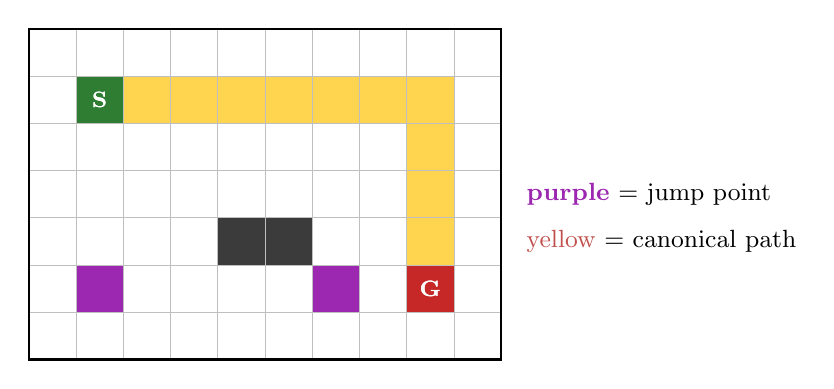
\begin{tikzpicture}[scale=1]
  \gridbase{10}{7}
  % wall
  \foreach \c in {4,5} { \fillcell{\c}{2}{wall} }
  % start and goal
  \fillcell{1}{5}{startc}\celltext{1}{5}{\textcolor{white}{\textbf{S}}}
  \fillcell{8}{1}{goalc}\celltext{8}{1}{\textcolor{white}{\textbf{G}}}
  % jump points (purple)
  \fillcell{1}{1}{jumpc}
  \fillcell{6}{1}{jumpc}
  % canonical path, horizontal first
  \foreach \c/\r in {2/5,3/5,4/5,5/5,6/5,7/5,8/5,8/4,8/3,8/2} {\fillcell{\c}{\r}{pathc}}
  \celltext{1}{5}{\textcolor{white}{\textbf{S}}}
  \celltext{8}{1}{\textcolor{white}{\textbf{G}}}
  \node[right=0.2cm] at (10*0.6,3.5*0.6) {\small \textcolor{jumpc}{\textbf{purple}} = jump point};
  \node[right=0.2cm] at (10*0.6,2.5*0.6) {\small \textcolor{accent2}{yellow} = canonical path};
\end{tikzpicture}
\end{center}

\noindent Without jumping, A* expands every yellow cell one at a time --- ten expansions. JPS4 expands only the start, the turning points, and the goal --- maybe three or four expansions. The yellow cells still appear in the final path (JPS4 fills them in at the end), but they were never in the priority queue.

\subsection{What JPS4 is good at and what it is not}

\begin{itemize}[leftmargin=20pt,itemsep=2pt]
  \item[\textcolor{accent}{\textbf{+}}] \textbf{Long open corridors.} This is where jumping shines: one jump can replace dozens of A* expansions.
  \item[\textcolor{accent}{\textbf{+}}] \textbf{Still optimal.} Baum proves (Theorem 4.2 in the paper) that JPS4 always returns a shortest path.
  \item[\textcolor{accent2}{\textbf{--}}] \textbf{Dense noise.} When obstacles are sprinkled everywhere (30\%+), corridors are short, so each ``jump'' barely advances, and the extra work of checking for forced neighbours at every step starts to hurt.
  \item[\textcolor{accent2}{\textbf{--}}] \textbf{Completely empty maps.} Surprisingly, A* can beat JPS4 on obstacle-free maps because the heuristic alone is enough to walk almost straight to the goal, and JPS4's per-step overhead is pure loss. This is the one result Baum warns about explicitly.
\end{itemize}

\clearpage
% ============================================================================
\section{A short summary of the research paper}\label{sec:paper}

\textbf{Title.}\enspace Jump Point Search Pathfinding in 4-connected Grids.\\
\textbf{Author.}\enspace Johannes Baum (Google), January 2025.\\
\textbf{Where.}\enspace arXiv preprint 2501.14816.

\subsection{The gap it fills}

The original Jump Point Search (JPS) was invented by Harabor and Grastien in 2011 for \textbf{8-connected} grids, where characters can move diagonally. But many video games and some robotics settings only allow the four cardinal directions (up, down, left, right) --- a \textbf{4-connected} grid. The original JPS does not work directly on 4-connected grids, because its pruning rules rely on diagonal moves to ``hop over'' corners of obstacles. Baum adapts the algorithm by replacing the 8-direction canonical ordering with a \textbf{horizontal-first} ordering and rewriting the natural- and forced-neighbour rules from scratch.

\subsection{What the paper contributes}

\begin{enumerate}[leftmargin=20pt,itemsep=2pt]
  \item A formal definition of the horizontal-first canonical ordering on 4-connected grids.
  \item New pruning rules (Algorithms 2 and 3 in the paper) that define natural and forced neighbours for only the four cardinal directions.
  \item A jump function (Algorithm 5) that returns immediately after one step for horizontal moves and recurses for vertical moves.
  \item A proof (Theorem 4.2) that JPS4 is optimal: it always returns a shortest path.
  \item Benchmarks on three real-world map sets from the Sturtevant pathfinding benchmark collection --- \textit{Dragon Age: Origins}, \textit{Baldur's Gate 2}, and \textit{Rooms} --- plus an empty-map set.
\end{enumerate}

\subsection{What the paper measures}

\begin{itemize}[leftmargin=20pt,itemsep=2pt]
  \item On \textbf{Baldur's Gate 2}, JPS4 is roughly \textbf{10--20$\times$} faster than A* for typical path lengths.
  \item On \textbf{Dragon Age: Origins}, about \textbf{10$\times$} faster.
  \item On \textbf{Rooms}, the speedup grows almost linearly with path length, reaching \textbf{50$\times$} or more.
  \item On an \textbf{empty map}, A* \emph{beats} JPS4. The empty-map speedup is less than 1.0 (around 0.03--0.14), because JPS4 visits every cell while A* walks almost straight to the goal.
\end{itemize}

Baum's conclusion is clear: JPS4 is a good drop-in for A* when your environment has meaningful obstacles, but on truly open terrain A* is still the right choice.

\begin{keybox}[One takeaway from the paper]
JPS4's speed comes from skipping symmetric paths through open corridors. The denser the ``useful'' structure of the map (rooms, walls, corridors), the more JPS4 wins. The sparser the structure, the less JPS4 wins --- and below a density threshold, A* wins.
\end{keybox}

\clearpage
% ============================================================================
\section{Project architecture: the code tour}\label{sec:arch}

Now that you understand the three algorithms, let's open the project and walk through every file. The top-level folder looks like this:

\begin{center}
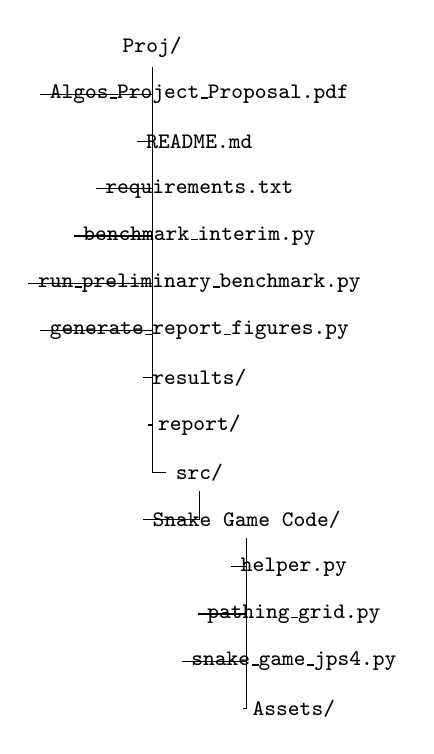
\begin{tikzpicture}[
  every node/.style={font=\footnotesize\ttfamily},
  grow via three points={one child at (0.6,-0.6) and two children at (0.6,-0.6) and (0.6,-1.2)},
  edge from parent path={(\tikzparentnode.south) |- (\tikzchildnode.west)}]
  \node[font=\footnotesize\ttfamily\bfseries] {Proj/}
    child { node {Algos\_Project\_Proposal.pdf} }
    child { node {README.md} }
    child { node {requirements.txt} }
    child { node {benchmark\_interim.py} }
    child { node {run\_preliminary\_benchmark.py} }
    child { node {generate\_report\_figures.py} }
    child { node {results/} }
    child { node {report/} }
    child { node {src/} child { node{Snake Game Code/}
      child { node{helper.py} }
      child { node{pathing\_grid.py} }
      child { node{snake\_game\_jps4.py} }
      child { node{Assets/} }
    }};
\end{tikzpicture}
\end{center}

\noindent The heart of the project is the three files inside \texttt{src/Snake Game Code/}. Everything else --- benchmarks, figure scripts, reports --- exists to drive or document those three files.

\subsection{The layered view}

\begin{center}
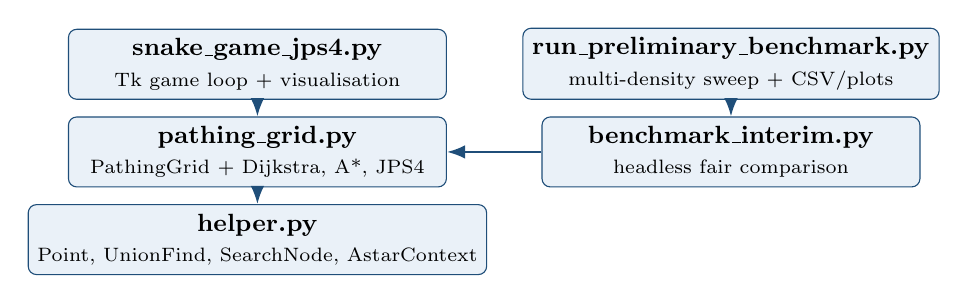
\begin{tikzpicture}[
  node distance=6pt,
  every node/.style={draw=accent,fill=soft2,rounded corners=3pt,minimum width=4.8cm,minimum height=0.8cm,align=center,font=\small},
  arr/.style={-Latex,thick,accent}]
  \node (h) {\textbf{helper.py}\\\scriptsize{Point, UnionFind, SearchNode, AstarContext}};
  \node (p) [above=of h] {\textbf{pathing\_grid.py}\\\scriptsize{PathingGrid + Dijkstra, A*, JPS4}};
  \node (g) [above=of p] {\textbf{snake\_game\_jps4.py}\\\scriptsize{Tk game loop + visualisation}};
  \node (b) [right=1.2cm of p] {\textbf{benchmark\_interim.py}\\\scriptsize{headless fair comparison}};
  \node (r) [above=of b] {\textbf{run\_preliminary\_benchmark.py}\\\scriptsize{multi-density sweep + CSV/plots}};
  \draw[arr] (p) -- (h);
  \draw[arr] (g) -- (p);
  \draw[arr] (b) -- (p);
  \draw[arr] (r) -- (b);
\end{tikzpicture}
\end{center}

Arrows read ``uses''. Higher boxes depend on lower boxes.

\subsection{\texttt{helper.py} --- the primitives}

This file defines the low-level pieces every search uses. Four things live here:

\paragraph{\texttt{Point}.}
A tiny class that holds an $(x, y)$ pair. It supports addition (\texttt{p1 + p2}), equality, hashing (so points can be used as dictionary keys), the four-cardinal neighbour list (\texttt{neumann\_neighborhood}), and the Manhattan distance. It has one subtle method, \texttt{direction\_to(other)}, which returns a unit-step direction $(dx, dy)$ --- used by JPS4 to figure out which way it is moving.

\paragraph{\texttt{UnionFind}.}
A classic data structure that answers the question ``are these two things in the same group?'' in almost constant time. The project uses it to pre-check whether the goal is even reachable from the start before running a search. If they are in different connected components of free cells, there is no point running Dijkstra/A*/JPS4 at all --- we already know the answer is ``no path''.

\paragraph{\texttt{SearchNode}.}
A lightweight record placed onto the priority queue. Holds four things:
\begin{itemize}[leftmargin=20pt,itemsep=1pt]
  \item \texttt{estimated\_cost} --- this is $f = g + h$. Python's heap orders on this first.
  \item \texttt{cost} --- this is $g$, used to break ties.
  \item \texttt{node} --- the actual grid cell.
  \item \texttt{parent} --- the cell we came from (for reconstructing the path at the end).
\end{itemize}

\paragraph{\texttt{AstarContext}.}
The generic best-first search loop, shared by all three algorithms. Its core is the method \texttt{astar\_jps(start, successors, heuristic, success)}. Read that signature carefully:

\begin{itemize}[leftmargin=20pt,itemsep=1pt]
  \item \texttt{start} --- where to begin.
  \item \texttt{successors(parent, current)} --- a \emph{function} that, given the current cell and its parent, returns the list of \texttt{(next\_cell, move\_cost)} tuples to try next. \textit{This is the knob that distinguishes Dijkstra/A*/JPS4.}
  \item \texttt{heuristic(cell)} --- a \emph{function} returning $h$. Dijkstra passes a function that always returns 0; A* and JPS4 pass a Manhattan-distance function.
  \item \texttt{success(cell)} --- a \emph{function} returning \texttt{True} if this cell is the goal.
\end{itemize}

By passing different functions for \texttt{successors} and \texttt{heuristic}, the same loop becomes Dijkstra, A*, or JPS4. The body of the loop is fewer than 20 lines.

\subsection{\texttt{pathing\_grid.py} --- the three algorithms}

This is the largest file in the project. It defines a \texttt{PathingGrid} class that holds the 2D boolean grid (\texttt{True} = blocked) and all three search implementations as methods. The structure:

\begin{center}
\renewcommand{\arraystretch}{1.2}
\begin{tabular}{@{}lp{10cm}@{}}
\toprule
\textbf{Method} & \textbf{What it does} \\
\midrule
\texttt{in\_bounds, get, set} & Grid bookkeeping. \\
\texttt{can\_move\_to(p)} & Is cell \texttt{p} inside and free? \\
\texttt{heuristic(p1, p2)} & Manhattan distance times the uniform cost. \\
\texttt{neighborhood\_points(p)} & The 4 cardinal neighbours of \texttt{p}. \\
\texttt{standard\_astar\_successors} & Returns all 4 free neighbours with cost 1. Used by Dijkstra and A*. \\
\texttt{jps\_prune\_neighbors} & Implements Baum's Algorithm 2 --- natural and forced neighbours. \\
\texttt{jps\_jump} & Implements Baum's Algorithm 5 --- horizontal returns after 1 step, vertical recurses until forced/goal/wall. \\
\texttt{jps\_successors} & Uses the previous two to produce the JPS4 successor list. \\
\texttt{reachable(a, b)} & Union-Find pre-check: are \texttt{a} and \texttt{b} in the same component? \\
\texttt{get\_waypoints\_single\_goal(s, g, mode)} & \textbf{The entry point.} Selects the right successor and heuristic functions based on \texttt{mode}, runs \texttt{astar\_jps}, measures time, records expansions, returns the path. \\
\texttt{get\_path\_single\_goal(s, g, mode)} & Thin wrapper that also validates the path. \\
\bottomrule
\end{tabular}
\end{center}

\subsection{\texttt{snake\_game\_jps4.py} --- the visual front-end}

This is a full Tkinter-based snake game. The snake's head is the \emph{start}, the food is the \emph{goal}, and the snake's body segments act like walls. Every time the game needs to decide the next move, it calls \texttt{PathingGrid.get\_path\_single\_goal} on the current board. The game also has a ``compare'' button that runs all three algorithms on the current state and draws each algorithm's chosen route in its own colour, so you can visually compare the three side by side:

\begin{center}
\renewcommand{\arraystretch}{1.2}
\begin{tabular}{@{}lll@{}}
\toprule
\textbf{Algorithm} & \textbf{Colour in the game} & \textbf{Source} \\
\midrule
Dijkstra & red-pink \texttt{\#d48888} & \texttt{COMPARE\_COLORS[0]} \\
A*       & green \texttt{\#88c488}    & \texttt{COMPARE\_COLORS[1]} \\
JPS4     & blue \texttt{\#6a9fd4}     & \texttt{COMPARE\_COLORS[2]} \\
\bottomrule
\end{tabular}
\end{center}

There are two built-in board layouts: an \textbf{easy} board with a few scattered walls (20$\times$20) and a \textbf{hard} board with a dense maze-like pattern. The hard board is where JPS4's advantage over A* is most visible.

\subsection{\texttt{benchmark\_interim.py} and \texttt{run\_preliminary\_benchmark.py}}

These two scripts drive \texttt{PathingGrid} headlessly (no GUI) and record CSVs of node expansions and wall-clock time for each algorithm.

\begin{itemize}[leftmargin=20pt,itemsep=2pt]
  \item \texttt{benchmark\_interim.py} runs a single density setting on a single grid size. It generates a random grid, picks a start and goal far apart, verifies they're connected, and runs all three algorithms on the \emph{same} instance so the comparison is fair.
  \item \texttt{run\_preliminary\_benchmark.py} imports the helpers from the interim script and runs multiple densities in a single pass, dumping CSV, JSON, a LaTeX table snippet, and matplotlib plots into \texttt{results/}.
\end{itemize}

\clearpage
% ============================================================================
\section{How a search call flows through the code}\label{sec:flow}

Let's trace what happens when the snake game asks for a path from head to food. This is the single most important flow in the project. Every number in the benchmark comes out of this sequence.

\begin{center}
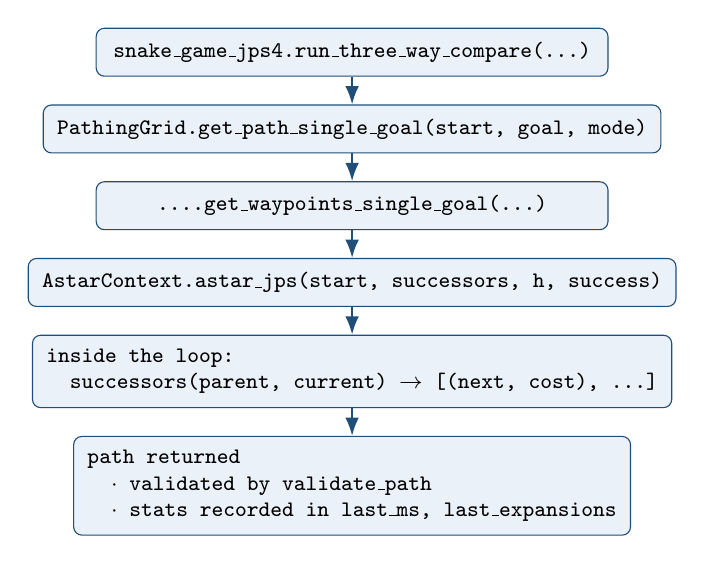
\begin{tikzpicture}[
  node distance=10pt and 12pt,
  every node/.style={draw=accent,rounded corners=3pt,fill=soft2,align=left,font=\footnotesize\ttfamily,inner sep=5pt,minimum width=6.5cm},
  arr/.style={-Latex,thick,accent}]
  \node (a) {snake\_game\_jps4.run\_three\_way\_compare(...)};
  \node (b) [below=of a] {PathingGrid.get\_path\_single\_goal(start, goal, mode)};
  \node (c) [below=of b] {\ldots.get\_waypoints\_single\_goal(\ldots)};
  \node (d) [below=of c] {AstarContext.astar\_jps(start, successors, h, success)};
  \node (e) [below=of d] {inside the loop:\\\hspace*{1em}successors(parent, current) $\to$ [(next, cost), \ldots]};
  \node (f) [below=of e] {path returned\\\hspace*{1em}$\cdot$\ validated by validate\_path\\\hspace*{1em}$\cdot$\ stats recorded in last\_ms, last\_expansions};
  \draw[arr] (a) -- (b);
  \draw[arr] (b) -- (c);
  \draw[arr] (c) -- (d);
  \draw[arr] (d) -- (e);
  \draw[arr] (e) -- (f);
\end{tikzpicture}
\end{center}

\subsection{Step-by-step in words}

\begin{enumerate}[leftmargin=20pt,itemsep=3pt]
  \item The game has the current head position, the current food position, and a 2D array of the board. It wants the shortest route from head to food that avoids the snake's own body.

  \item The game builds a fresh \texttt{PathingGrid} for this moment in time, marks the body segments as blocked, and calls \texttt{get\_path\_single\_goal(head, food, mode)}. The \texttt{mode} string is one of \texttt{"dijkstra"}, \texttt{"astar"}, or \texttt{"jps4"}.

  \item \texttt{get\_path\_single\_goal} resets the measurement counters (\texttt{last\_ms} and \texttt{last\_expansions}) and calls \texttt{get\_waypoints\_single\_goal}, which does three cheap checks first:
    \begin{itemize}[leftmargin=14pt,itemsep=1pt]
      \item If start and goal are adjacent, return \texttt{[start, goal]} immediately.
      \item If there's a straight unobstructed line between them, return that line.
      \item Otherwise, run the union-find \texttt{reachable} check. If the two cells are in different connected components, return \texttt{None} (no path).
    \end{itemize}

  \item If all the cheap checks fail, we run the search. Here is the key moment where the algorithm is chosen, and it is essentially three lines:
\begin{lstlisting}[language=Python]
if mode == "jps4":
    result = context.astar_jps(start,
        lambda p, n: self.jps_successors(p, n, goal_test),
        heuristic, goal_test)
elif mode == "dijkstra":
    result = context.astar_jps(start,
        lambda p, n: self.standard_astar_successors(n, goal_test),
        lambda _: 0,  # heuristic = 0
        goal_test)
else:   # "astar"
    result = context.astar_jps(start,
        lambda p, n: self.standard_astar_successors(n, goal_test),
        heuristic, goal_test)
\end{lstlisting}

  \item \texttt{astar\_jps} runs the generic best-first search loop: it pops the lowest-$f$ node, checks if it's the goal, otherwise asks the \texttt{successors} function for children, relaxes their costs, and pushes them onto the priority queue. It increments \texttt{expansions} by 1 for each pop.

  \item When the goal pops out of the queue, \texttt{astar\_jps} walks back through the \texttt{parents} dictionary to reconstruct the path, and returns it.

  \item \texttt{get\_waypoints\_single\_goal} records the wall-clock time (\texttt{last\_ms}) and the expansion count (\texttt{last\_expansions}), then runs one final validation pass --- checking that every pair of adjacent points in the path is actually adjacent on the grid and not blocked.

  \item Control returns to the caller. The snake game paints the path, or the benchmark script writes one row into the CSV.
\end{enumerate}

That's the entire pipeline. Once you've followed it once end-to-end, reading any individual file in the project becomes much easier.

\clearpage
% ============================================================================
\section{The Snake game, in detail}\label{sec:game}

The Snake game is not just decoration --- it is a live laboratory. Every time the snake grows by one segment, the game calls the pathfinder again, because the blocked-cell map has changed. Watching the snake play on the hard board is a visceral way to see how an algorithm behaves when obstacles are constantly appearing and disappearing.

\subsection{The game grid}

The game uses a fixed 20$\times$20 grid. Each cell has a numeric label:

\begin{center}
\begin{tabular}{@{}cl@{}}
\toprule
\textbf{Value} & \textbf{Meaning} \\
\midrule
0 & EMPTY --- walkable \\
1 & BODY --- snake body segment (blocks the pathfinder) \\
2 & FOOD --- the goal \\
3 & HEAD --- the snake's head (the start) \\
4 & WALL --- permanent wall from the board layout \\
\bottomrule
\end{tabular}
\end{center}

\subsection{The tick cycle}

Every game tick:

\begin{enumerate}[leftmargin=20pt,itemsep=2pt]
  \item Copy the 2D board.
  \item Temporarily remove the tail cell (it will move forward next, so it is actually free this tick).
  \item Build a \texttt{PathingGrid} and mark all WALL and BODY cells as blocked.
  \item Call \texttt{pg.get\_path\_single\_goal(head, food, mode=current\_mode)}.
  \item Take the first step of the returned path and move the snake head there.
  \item If the new head lands on food, grow the snake by one segment and spawn new food.
  \item Record timing and expansion counts for the HUD.
\end{enumerate}

\subsection{The compare mode}

The game has a button that runs \emph{all three} algorithms on the current board state and draws each returned path in its own colour. The helper \texttt{run\_three\_way\_compare} does exactly this. When the three paths are equal length (the common case), what differs is not the route but the \emph{effort} it took to compute each route --- which is exactly what the HUD reports: per-algorithm running totals of node expansions and wall-clock time.

\subsection{The two boards}

The file \texttt{snake\_game\_jps4.py} defines two hand-drawn boards:

\begin{itemize}[leftmargin=20pt,itemsep=2pt]
  \item \texttt{EASY\_BOARD\_LAYOUT} --- a 20$\times$20 board with a thin wall around the outside and only a handful of interior obstacles.
  \item \texttt{HARD\_BOARD\_LAYOUT} --- a 20$\times$20 board with many interior walls forming a maze. This is the board that makes JPS4 look good.
\end{itemize}

\subsection{Why the snake game is a good demo for JPS4}

\begin{enumerate}[leftmargin=20pt,itemsep=2pt]
  \item The snake's own body is a constantly-changing obstacle. This forces a fresh search every tick, so the per-search cost is what matters.
  \item On the hard board, the maze structure creates many long corridors --- exactly the pattern JPS4 is tuned for.
  \item You can watch the per-algorithm HUD counters grow in real time as the snake plays, which makes the ``expansions'' metric concrete.
\end{enumerate}

\clearpage
% ============================================================================
\section{The benchmarking methodology}\label{sec:bench}

The benchmark scripts exist to answer the question: \emph{across many random grids, which algorithm is fastest and by how much?}

\subsection{Fair comparison}

The single most important rule in benchmarking: \textbf{the same instance must be fed to all three algorithms}. If Dijkstra got an easier random grid than A*, the comparison is meaningless. The code honours this rule by generating a grid once, verifying it is solvable, and then running all three algorithms on that same grid back-to-back before moving on to the next grid.

\subsection{What each script does}

\paragraph{\texttt{benchmark\_interim.py}.}
Single-density run. Default parameters: 50$\times$50 grid, density 0.28 (28\% of cells blocked), 40 trials, seed 42. It writes two files into \texttt{results/}:
\begin{itemize}[leftmargin=20pt,itemsep=1pt]
  \item a CSV with one row per (trial, algorithm),
  \item a short text summary with mean and standard deviation per algorithm.
\end{itemize}

\paragraph{\texttt{run\_preliminary\_benchmark.py}.}
Sweeps density values and records the results for a progress-report-style table. Writes CSV + JSON + a LaTeX table snippet + matplotlib PNGs. This is what produced the \textit{results\_combined.png} figure used in the interim progress report.

\subsection{Start and goal placement}

The helper \texttt{pick\_start\_goal} samples random pairs of free cells and keeps the pair with the largest Manhattan distance. This biases the benchmark toward \emph{long} problems, which is where any pathfinder's differences are visible. Very short problems all finish in microseconds and tell us nothing.

\subsection{What is reported}

For each trial, three numbers:

\begin{itemize}[leftmargin=20pt,itemsep=2pt]
  \item \textbf{\texttt{ms}} --- wall-clock time in milliseconds for the search call.
  \item \textbf{\texttt{expansions}} --- number of cells popped out of the priority queue. This is the cleanest metric.
  \item \textbf{\texttt{path\_cells}} --- number of cells in the final path. \emph{All three algorithms should produce the same number} on every trial; if they don't, something is wrong with one of the implementations.
\end{itemize}

\subsection{What the interim numbers showed}

On 50$\times$50 grids with the JPS4 implementation corrected to match Baum's pruning rules, you should expect roughly:

\begin{center}
\renewcommand{\arraystretch}{1.25}
\begin{tabular}{@{}lrrrrrr@{}}
\toprule
& \multicolumn{2}{c}{\textbf{15\% blocked}} & \multicolumn{2}{c}{\textbf{28\% blocked}} & \multicolumn{2}{c}{\textbf{40\% blocked}} \\
\cmidrule(lr){2-3}\cmidrule(lr){4-5}\cmidrule(lr){6-7}
& Exp. & ms & Exp. & ms & Exp. & ms \\
\midrule
Dijkstra & $\sim$2000 & $\sim$7 & $\sim$1700 & $\sim$5 & $\sim$900 & $\sim$3 \\
A*       & $\sim$1000 & $\sim$4 & $\sim$630  & $\sim$2 & $\sim$510 & $\sim$2 \\
JPS4     & $\sim$490  & $\sim$4 & $\sim$380  & $\sim$3 & $\sim$320 & $\sim$2 \\
\bottomrule
\end{tabular}
\end{center}

\noindent (The JPS4 numbers above assume the corrected pruning rules from \S\ref{sec:jps}. With the earlier buggy version, JPS4's expansions were artificially inflated at higher densities because the fallback hacks kicked in.)

On wall-clock time, Python's interpreter overhead makes JPS4 look worse than its expansion count alone suggests --- its inner loop is more complex. Baum's paper, running on Node.js with a tighter implementation, shows $10$--$20\times$ speed-ups on real game maps; in Python the ratio is smaller but the expansion-count story is the same.

\clearpage
% ============================================================================
\section{Glossary}
\addcontentsline{toc}{section}{Glossary}

\begin{description}[leftmargin=130pt, style=nextline]
  \item[\textbf{Admissible heuristic}] A heuristic $h$ that never over-estimates the true remaining cost to the goal. Makes A* optimal.
  \item[\textbf{A*}] A best-first search that uses $f = g + h$ as the priority. Always optimal when $h$ is admissible.
  \item[\textbf{Best-first search}] A search that always expands the frontier cell with the smallest priority next. Dijkstra, A*, and JPS4 are all best-first searches.
  \item[\textbf{Canonical ordering}] An artificial rule that forces a unique shortest path among many equivalent ones. JPS4 uses ``horizontal first''.
  \item[\textbf{Dijkstra's algorithm}] A best-first search where the priority is just $g$. No heuristic.
  \item[\textbf{Expansion}] One pop from the priority queue and the work of generating its successors. The main efficiency metric.
  \item[\textbf{$f$}] The priority number on the queue. $f = g + h$ in A* and JPS4; $f = g$ in Dijkstra.
  \item[\textbf{Forced neighbour}] In JPS4, a neighbour that would normally be pruned but must be kept because an adjacent cell is blocked. A wall has ``broken the symmetry''.
  \item[\textbf{Frontier} (open list)] The set of cells waiting to be expanded. Implemented as a priority queue.
  \item[\textbf{$g$}] The running cost from the start to the current cell. In 4-connected grids with uniform cost, this is just the step count.
  \item[\textbf{Graph}] A set of nodes (dots) connected by edges (lines). A grid becomes a graph where free cells are nodes and adjacency gives edges.
  \item[\textbf{$h$}] The heuristic --- a guess of the remaining cost to the goal. Manhattan distance on 4-connected grids.
  \item[\textbf{Horizontal-first JPS (HJPS/JPS4)}] Baum's 2025 adaptation of Jump Point Search for 4-connected grids using a horizontal-first canonical ordering.
  \item[\textbf{Jump point}] In JPS4, a cell where the search must stop and record a new open-list entry: either the goal, or a cell with at least one forced neighbour, or any cell reached via a horizontal move.
  \item[\textbf{Manhattan distance}] $|x_1 - x_2| + |y_1 - y_2|$. The minimum number of 4-connected steps between two cells in an obstacle-free grid.
  \item[\textbf{Natural neighbour}] A neighbour that the canonical ordering keeps by default.
  \item[\textbf{Path-symmetry problem}] The observation that on open 4-connected grids there are many shortest paths and most of them differ only by the order of the moves.
  \item[\textbf{Priority queue}] A container that always returns the item with the smallest priority. Python's \texttt{heapq} module.
  \item[\textbf{Pruning}] Skipping the generation of successors that cannot possibly lie on a canonical shortest path.
  \item[\textbf{Union-Find}] A data structure that answers ``are these two cells in the same connected region?'' in near-constant time.
  \item[\textbf{Uniform-cost grid}] A grid where every step has the same cost. All the grids in this project are uniform-cost.
\end{description}

\vspace{1em}
\begin{center}
\itshape End of guide. Return to the code with confidence.\par
\small See \texttt{pathing\_grid.py} and \texttt{helper.py} for the implementations described here,\\
and \texttt{benchmark\_interim.py} to reproduce the numbers in \S\ref{sec:bench}.
\end{center}

\end{document}
